%%% template.tex
%%%
%%% This LaTeX source document can be used as the basis for your technical
%%% paper or abstract.

%%% The parameter to the ``documentclass'' command is very important.
%%% - use ``review'' for content submitted for review.
%%% - use ``preprint'' for accepted content you are making available.
%%% - use ``tog'' for technical papers accepted to the TOG journal and
%%%   for presentation at the SIGGRAPH or SIGGRAPH Asia conference.
%%% - use ``conference'' for final content accepted to a sponsored event
%%%   (hint: If you don't know, you should use ``conference.'')

\documentclass[review]{acmsiggraph}
\usepackage{amsmath}
\usepackage{amssymb}
\usepackage{wasysym}
\usepackage[scaled=.92]{helvet}
\usepackage{times}
\usepackage{graphicx}
\usepackage{parskip}
\usepackage{url}
\usepackage[labelfont=bf,textfont=it]{caption}
\usepackage{color}
\usepackage{algorithm}
\usepackage{algorithmic}
\usepackage{enumitem}
\usepackage{authblk}

%----------------------------------------------------------------------------
%----------------------------------------------------------------------------
\definecolor{AdamColor}{rgb}{0,0,0.7}
\definecolor{BenColor}{rgb}{0,0.7,0}
\definecolor{tamarColor}{rgb}{0.8,0,0.8}
\definecolor{JoshColor}{rgb}{0.0,0.7,0.8}
\newcommand{\mycomment}[1]{}
\newcommand{\adam}[1]{{\color{AdamColor} #1}}
\newcommand{\ben}[1]{{\color{BenColor} #1}}
\definecolor{nilsCol}{rgb}{0.85,0.35,0.25}
\newcommand{\Nils}[1]{\textcolor{nilsCol}{#1}}
\newcommand{\tamar}[1]{\textcolor{tamarColor}{#1}}
\newcommand{\josh}[1]{\textcolor{JoshColor}{#1}}
% for final
%\newcommand{\adam}[1]{{#1}}
%\newcommand{\Nils}[1]{{#1}}

%\let\shortcite=\cite
%\newcommand{\shortcite}[1]{\cite{#1}}
\newcommand{\etal}{and colleagues}
\newcommand{\Mueller}{M\"uller~}
\newcommand{\BM}[1]{\B{#1}}
%\newcommand{\B}[1]{\mbox{\boldmath$#1$}}
%\newcommand{\B}[1]{\textbf{\textit{#1}}}
\newcommand{\B}[1]{\mathit{\mathbf{#1}}}
\newcommand{\Per}{\%}
\newcommand{\Unit}[1]{{\mbox{$\,\mathrm{#1}$}}}
\newcommand{\Snit}[1]{{\mbox{\small$\mathrm{#1}$}}}
\newcommand{\Tr}[1]{\mathrm{Tr}\left(#1\right)}
\newcommand{\sign}[1]{\mathrm{sign}\left(#1\right)}
\newcommand{\Hz}{\Unit{Hz}}
\newcommand{\MHz}{\Unit{MHz}}
\newcommand{\GHz}{\Unit{GHz}}
\newcommand{\Sec}{\Unit{sec}}
\newcommand{\SPF}{\Unit{sec/frame}}
\newcommand{\Min}{\Unit{min}}
\newcommand{\Max}{\Unit{max}}
\newcommand{\M}{\Unit{m}}
\newcommand{\Nab}{\B{\nabla}}
\newcommand{\TP}{^\mathsf{T}}

\newcommand{\Dist}{\mbox{dist}}

\newcommand{\figureTopBot}[1]{
  \begin{figure}[!tb]{\sloppy #1}\end{figure}
}

\newcommand{\figureTop}[1]{
  \begin{figure}[!t]{\sloppy #1}\end{figure}
}
 
\newcommand{\figureBot}[1]{
  \begin{figure}[!b]{\sloppy #1}\end{figure}
}

\newcommand{\figureWideTop}[1]{
  \begin{figure*}[!t]{\sloppy #1}\end{figure*}
}

\newcommand{\figureWideBot}[1]{
  \begin{figure*}[!b]{\sloppy #1}\end{figure*}
}

\newcommand{\eqAlgn}{\!\!&\!\!}

\newcommand{\Eref}[1]{Equation~(\ref{#1})}
\newcommand{\Erefs}[2]{Equations~(\ref{#1}) and (\ref{#2})}
\newcommand{\eref}[1]{Equation~(\ref{#1})}
\newcommand{\erefs}[2]{Equations~(\ref{#1}) and (\ref{#2})}
\newcommand{\Sref}[1]{Section~\ref{#1}}
\newcommand{\sref}[1]{Section~\ref{#1}}
\newcommand{\srefs}[2]{Sections~\ref{#1} and~\ref{#2}}
\newcommand{\fref}[1]{Figure~\ref{#1}}
\newcommand{\frefAND}[2]{Figures~\ref{#1} and~\ref{#2}}
\newcommand{\frefs}[2]{Figures~\ref{#1} and~\ref{#2}}
\newcommand{\frefss}[3]{Figures~\ref{#1}, \ref{#2}, and~\ref{#3}}
\newcommand{\frefsss}[4]{Figures~\ref{#1}, \ref{#2}, \ref{#3}, and~\ref{#4}}
\newcommand{\Fref}[1]{Figure~\ref{#1}}
\newcommand{\Frefs}[2]{Figures~\ref{#1} and~\ref{#2}}
\newcommand{\Frefss}[3]{Figures~\ref{#1}, \ref{#2}, and~\ref{#3}}
\newcommand{\Frefsss}[4]{Figures~\ref{#1}, \ref{#2}, \ref{#3}, and~\ref{#4}}
\newcommand{\tref}[1]{Table~\ref{#1}}

\renewcommand{\labelenumi}{\arabic{enumi}.}
\renewcommand{\labelenumii}{\alph{enumii}.}
\renewcommand{\labelenumiii}{\roman{enumiii}.}

\newenvironment{algstep}{%
  \begin{enumerate}%
    \setlength{\itemsep}{0in}%
    \setlength{\partopsep}{0in}%
    \setlength{\topsep}{0in}%
}{\end{enumerate}}

%----------------------------------------------------------------------------
%----------------------------------------------------------------------------

%%% Make the ``BibTeX'' word pretty...

\def\BibTeX{{\rm B\kern-.05em{\sc i\kern-.025em b}\kern-.08em
    T\kern-.1667em\lower.7ex\hbox{E}\kern-.125emX}}

%%% Used by the ``review'' variation; the online ID will be printed on 
%%% every page of the content.

\TOGonlineid{}

%%% Used by the ``preprint'' variation.

\TOGvolume{0}
\TOGnumber{0}

\title{Ductile Fracture for Clustered Shape Matching}
\author[*]{Ben Jones}
\author[**]{Joshua A. Levine}
\author[***]{Tamar Shinar}
\author[*]{Adam W. Bargteil}
\affil[*]{University of Utah}
\affil[**]{Clemson University}
\affil[***]{University of California, Riverside}
\pdfauthor{}

\keywords{Shape Matching, Ductile Fracture}

\begin{document}

%%% This is the ``teaser'' command, which puts an figure, centered, below 
%%% the title and author information, and above the body of the content.

 \teaser{
   %\includegraphics[height=1.5in]{Figures/}
   \caption{}
 }

\maketitle

\begin{abstract}
In this paper, we introduce incorporate ductile fracture into the clustered shape matching simulation framework
for deformable bodies, thus filling a gap in the shape matching literature.  The resulting approach is fast,
versatile, and simple to implement.
\end{abstract}

\begin{CRcatlist}
  \CRcat{I.3.7}{Computer Graphics}{Three-Dimensional Graphics and Realism}{Animation};
  \CRcat{I.6.8}{Simulation and Modeling}{Types of Simulation}{Animation}.
\end{CRcatlist}

\keywordlist

%% Required for all content. 

\copyrightspace

\section{Introduction}\label{sec:Introduction}
{\em Shape matching} is a geometrically motivated technique for animating deformable bodies introduced
a decade ago by \Mueller and colleagues~\shortcite{Mueller:2005:MDB}.
\fref{fig:shapematching} summarizes the approach.
In their seminal work, \Mueller and colleagues~\shortcite{Mueller:2005:MDB} introduced a simple plasticity
model and, in follow up work, Rivers and James~\shortcite{Rivers:2007:FFL}
incorporated a simple fracture model.  However, ductile fracture has not yet been addressed in the
shape matching literature.

\begin{figure*}
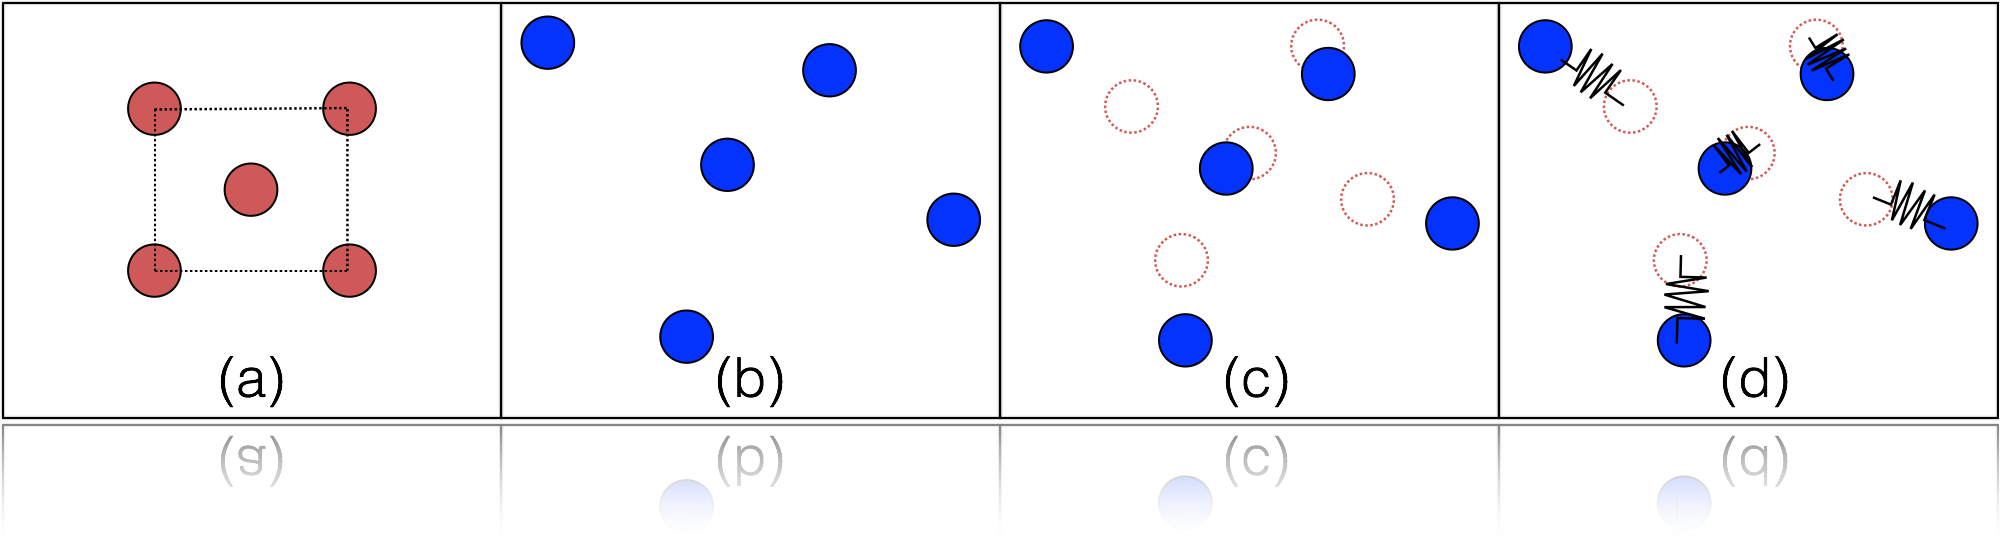
\includegraphics[width=\linewidth]{Figures/shapematching.png}
\caption{Shape Matching Overview: (a) An object (here, a square) is sampled with particles, $p_i$, to get rest positions, $\B{r}_i$.  
(b) As particles are subjected to external forces and constraints, their positions, $\B{x}_i$, are updated in world space.  
(c)  The best-fitting rigid transformation of the particles' rest positions, $\B{r}_i$, 
to their world positions, $\B{x}_i$ is computed.  The dotted red circles are the {\em goal} positions, $\B{g}_i$.  
(d) Hookean springs pull the world positions toward the goal positions.}
\label{fig:shapematching}
\end{figure*}

%In this paper, we incorporate ductile fracture into the clustered shape matching simulation framework
%for deformable bodies, thus filling a gap in the shape matching literature. 
In this paper, we enable the animation of ductile fracture 
by incorporating plasticity and fracture models into the clustered shape matching framework.
Our models are inspired by finite element approaches to animating deformable bodies, but are adapted to 
clustered shape matching.
Specifically, inspired by the work of Irving and colleagues~\shortcite{Irving:2004:IFE} and Bargteil and 
colleagues~\shortcite{Bargteil:2007:AFE}, we introduce a multiplicative plasticity model that incorporates
yield stress, flow rate, and work hardening.  Inspired by the work of O'Brien and colleagues~\shortcite{Obrien:1999:GMA,Obrien:2002:GMA},
we introduce a cluster-based fracture approach that splits individual clusters along the plane orthogonal to the direction the 
cluster is most stretched.
Taken together these contributions allow animation of ductile in the clustered shape matching framework.

\section{Related Work}
The geometrically motivated shape matching approach was introduced by \Mueller and 
colleagues~\shortcite{Mueller:2005:MDB}, who demonstrated impressive results and 
described the key advantages of the approach: efficiency, stability, and controllability.
Given these advantages, shape matching is especially appealing in interactive animation contexts such 
video games.  The authors also introduced several extensions including linear and quadratic deformations 
(in addition to rigid deformations), cluster-based deformation, and plasticity.  

Two years later, Rivers and James~\shortcite{Rivers:2007:FFL} introduced lattice-based shape matching,
which used a set of hierarchical lattices to define the shape matching clusters.  They took advantage
of the regular structure of the lattices to achieve extremely high performance.  They also incorporated a 
simple fracture model that removed over-extended links in the lattice.  

Since this time, the shape matching framework has been largely disregarded by the research community in favor of position-based
dynamics~\cite{Mueller:2007:PBD,Bender:2013:PBM,Bender:2014:ASO,Macklin:2014:UPP}.  One notable exception is
the work of Bargteil and Jones~\shortcite{Bargteil:2014:SLF}, which incorporated strain-limiting into clustered shape matching.
We incorporate our ductile fracture approach into their framework.

Ductile fracture is distinguished from brittle fracture by the inclusion plastic deformation.  Materials undergoing ductile
fracture (e.g. play dough) appear to {\em tear}, while brittle materials (e.g. glass) appear to {\em shatter}.  Most
real-world materials demonstrate some amount of plastic deformation during failure, so purely brittle models have fairly limited
application in computer animation.  
Both plasticity and fracture
were first demonstrated in computer animation by the pioneering work of Terzopoulos and Fleischer~\shortcite{Terzopoulos:1988:MID}; 
however, it was O'Brien and colleagues~\shortcite{Obrien:2002:GMA}
who first combined these phenomena to animate ductile fracture.  Since that time, plasticity and fracture have
remained very active research areas in computer animation and a thorough review is beyond the scope of this short paper.
\adam{in part this is because I am lazy, does anyone think it would be important?}

Our approach 
to fracture closely resembles that of O'Brien and colleagues~\shortcite{Obrien:1999:GMA,Obrien:2002:GMA}; however, instead of splitting tetrahedra,
we split shape matching clusters.  Our plasticity model closely resembles that of Bargteil and colleagues~\shortcite{Bargteil:2007:AFE}, except that
we apply it to shape matching clusters instead of individual tetrahedra and make no particular effort to ensure that plastic deformation does not
lead to insability, i.e. we do not update clusters to ensure well-conditioned matrices as done by, for example, Jones and colleagues~\shortcite{Jones:2014:DEF}.

\section{Methods}
\subsection{Shape Matching}
In the shape matching framework
objects are discretized into a set of particles, $p_i\in\mathcal{P}$, with rest positions, $\B{r}_i$, 
that follow a path, $\B{x}_i(t)$, in world-space through time.  
At each frame, shape matching solves for the rotation matrix, $\B{R}$, and a translation
vector, $\B{x}_{cm}-\B{r}_{cm}$, that minimize
\begin{equation}
\sum_i \left(\B{R}\left(\B{r}_i - \B{r}_{cm}\right)-\left(\B{x}_i-\B{x}_{cm}\right)\right)^2.
\end{equation}
The best translations are given by the center-of-mass in the rest and world space, respectively.  
The rotation, $\B{R}$, is computed through a polar decomposition.  Intuitively, this computation
yields the least-squares best-fit rigid transformation from the rest pose to the current deformed pose.
This transformation allows us to define goal positions, $\B{g}_i$,
\begin{equation}
\B{g}_i = \B{R}\left(\B{r}_i-\B{r}_{cm}\right)+\B{x}_{cm}.
\end{equation}
Hookean springs are then used to define forces that move the particles toward the goal positions.

More specifically, we first compute the least-squares best-fit linear deformation gradient as
\begin{equation}
\B{F} = \left(\sum_i m_i \B{O}(\B{x}_i,\B{r}_i)\right)\left(\sum_im_i\B{O}(\B{r}_i,\B{r}_i)\right)^{-1},
\end{equation}
where $\B{O}(\cdot,\cdot)$ is the outer product matrix
\begin{equation}
\B{O}(\B{a}_i,\B{b}_i) = \left(\B{a}_i-\B{a}_{cm}\right)\left(\B{b}_{i}-\B{b}_{cm}\right)^T
\end{equation}
%\begin{align}
%\B{F} = &\left(\sum_i m_i\left(\B{x}_{i}-\B{x}_{cm}\right)\left(\B{r}_{i}-\B{r}_{cm}\right)^T\right)\notag\\
%&\left(\sum_i m_i\left(\B{r}_{i}-\B{r}_{cm}\right)\left(\B{r}_{i}-\B{r}_{cm}\right)^T\right)^{-1},
%\end{align}
and $m_i$ is the mass of $p_i$.  $\B{F}$ minimizes
\begin{equation}
\sum_i \left(\B{F}\left(\B{r}_i - \B{r}_{cm}\right)-\left(\B{x}_i-\B{x}_{cm}\right)\right)^2.
\end{equation}
We then compute $\B{R}$ using the polar decomposition,
\begin{equation}
\B{F} = \B{R}\B{S} = \left(\B{UV}^T\right)\left(\B{V\Sigma V}^T\right)
\end{equation}
where $\B{S}=\B{V\Sigma V}^T$ is a symmetric matrix and $\B{U\Sigma V}^T$ is the singular value decomposition (SVD) of $F$.
While several researchers have pointed out that the polar decompositions can be computed faster than the SVD,
especially when warm started, we use the the SVD for its robustness and for our plasticity and fracture models
that follow.  We also note that we compute the rotation from 

%This basic approach was extended by including linear and quadratic global deformations, cluster-based
%deformations, and plasticity.


\section{Results and Discussion}

\paragraph{Limitations}

\section*{Acknowledgements}
Removed for anonymous review.

\bibliographystyle{acmsiggraph}
\bibliography{csm}
\end{document}
